
\graphicspath{ {chapters/Matemáticas/Sistema de coordenadas/images/} }

\chapter{Coordenadas Curvilíneas Ortogonales }

Clase 1

Los sistemas de coordenadas curvilíneas ortogonales hacen referencia a puntos en el espacio determinados por el corte de tres superficies, tales que, los vectores unitarios tangentes a cada curva de la intersección de dos de ellos son ortogonales entre sí.

Como ejemplo, revisemos que ocurre en las coordenadas cartesianas. Allí, cada punto espacial es determinado por la intersección de tres planos mutuamente ortogonales entre sí y que adicionalmente los tres vectores unitarios $\hat{i}, \hat{j}, \hat{k}$ permanecerán siendo los mismos mediante una operación de traslación de ellos al punto en consideración.

\begin{center}
  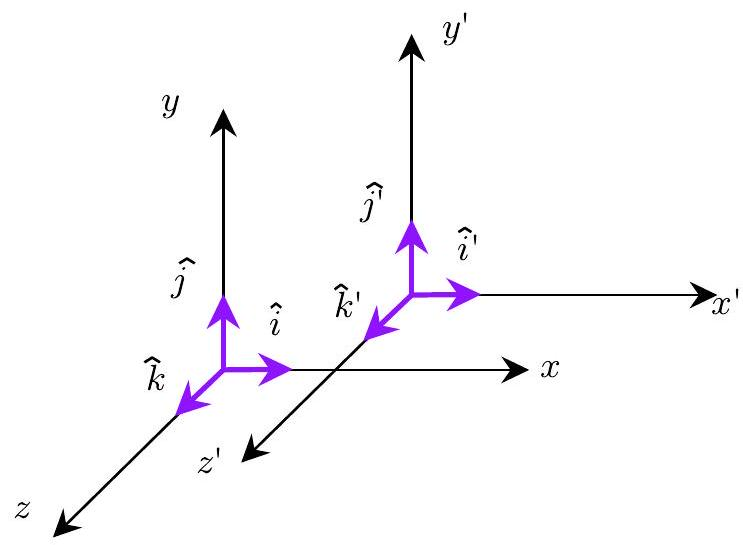
\includegraphics[max width=\textwidth]{sistemas_coordenados.jpg}
\end{center}

De tal forma que $\hat{i}=\hat{i}^{\prime}, \hat{j}=\hat{j}^{\prime}, \hat{k}=\hat{k}^{\prime}$

Miremos ahora que sucede en coordenadas cilíndricas. En este caso, las tres superficies que se intersectan son:

\begin{itemize}
  \item Un cilindro, un plano y un semiplano, De esta manera las tres nuevas variables serán: $\rho$ el radio del cilindro, $\theta$ el ángulo de apertura del semiplano y $z$ la posición del plano. Observemos esto en la siguiente figura:
\end{itemize}

\begin{center}
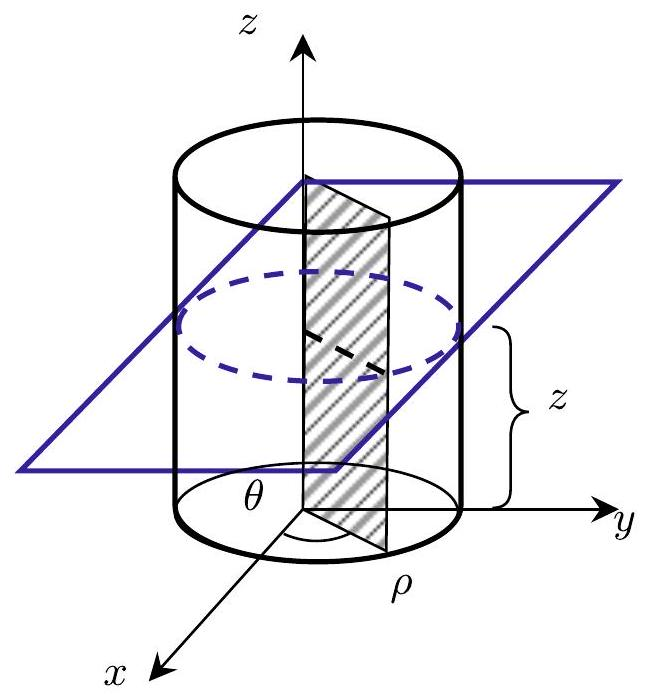
\includegraphics[max width=\textwidth]{/home/gabo/Documents/PLNotes/chapters/Matemáticas/Sistema de coordenadas/images/2023_01_14_5f03f91587087c6429b1g-1(1).jpg}
\end{center}

Como se evidencia en la figura, la curva producto del corte entre el cilindro y el semiplano es una línea recta vertical, que determinará la coordenada $z$; la curva determinada por el corte del semiplano y el plano, determinará una semirecta que será $\rho$ y por último el corte entre el plano y el cilindro, será una circunferencia, que determinará $\theta$. De esta forma los tres vectores unitarios ortogonales entre sí y tangentes a estas curvas, serán:

$\hat{e}_{\rho}:$ vector tangente a la semirecta

$\hat{e}_{\theta}$ : vector tangente a la circunferencia

$\hat{e}_{z}$ : vector tangente a la recta vertical

Ellos forman entre sí un conjunto de mano derecha, por lo tanto

$$
\hat{e}_{\rho}=\hat{e}_{\theta} \times \hat{e}_{z}, \quad \hat{e}_{z}=\hat{e}_{\rho} \times \hat{e}_{\theta}, \quad \widehat{e}_{\theta}=\hat{e}_{z} \times \hat{e}_{\rho} .
$$

Adicionalmente, la propiedad de ortogonalidad la evidencio como:

$$
\widehat{e}_{\rho} \cdot \widehat{e}_{\theta}=\widehat{e}_{\rho} \cdot \widehat{e}_{z}=\widehat{e}_{\theta} \cdot \hat{e}_{z}=0
$$

Por último, como ejemplo, revisemos el caso de las coordenadas esféricas. En este caso las superficies que se intersectan son: una esfera, un semiplano y un tronco de cono.

Las respectivas curvas que se producen son:

\begin{itemize}
  \item De la intersección del tronco de cono y la esfera, una circunferencia.

  \item Del cono y el semiplano una semirecta.

  \item Del semiplano y la esfera, una semicircunferencia.

\end{itemize}

Lo que determina tres vectores unitarios ortogonales

$\hat{e}_{r}$ : vector tangente a la semirecta

$\hat{e}_{\theta}$ : vector tangente a la semicircunferencia

$\hat{e}_{\varphi}:$ vector tangente a la circunferencia

y las tres variables $r, \theta, \varphi$.

De nuevo este conjunto de vectores unitarios forman un conjunto de mano derecha, por lo tanto:

$$
\widehat{e}_{r}=\widehat{e}_{\theta} \times \hat{e}_{\varphi}, \hat{e}_{\varphi}=\widehat{e}_{r} \times \widehat{e}_{\theta}, \widehat{e}_{\theta}=\hat{e}_{\varphi} \times \hat{e}_{r}
$$

Debe notarse muy especialmente que en cualquier sistema de coordenadas curvilíneas ortogonales que no sea el cartesiano, la dirección de los vectores unitarios cambia punto a punto. Este hecho es importante, pues, mientras los vectores $\hat{i}, \hat{j}, \hat{k}$ no varían punto a punto, los otros si lo harán. Para los dos últimos casos mencionados debe tenerse en cuenta que las respectivas transformaciones de coordenadas entre estos sistemas y el cartesiano, son:

\begin{center}
\begin{tabular}{|l|l|}
\hline
Cilíndricas & Esféricas \\
\hline
\end{tabular}
\end{center}

$$
x=\rho \cos \theta, y=\rho \sin \theta, z
$$

$$
\begin{aligned}
& x=r \sin \theta \cos \varphi \\
& y=r \sin \theta \sin \varphi \\
& z=r \cos \theta
\end{aligned}
$$

Dentro del espacio Euclideo, se reconocen los siguientes sistemas de coordenadas curvilíneas ortogonales

\begin{center}
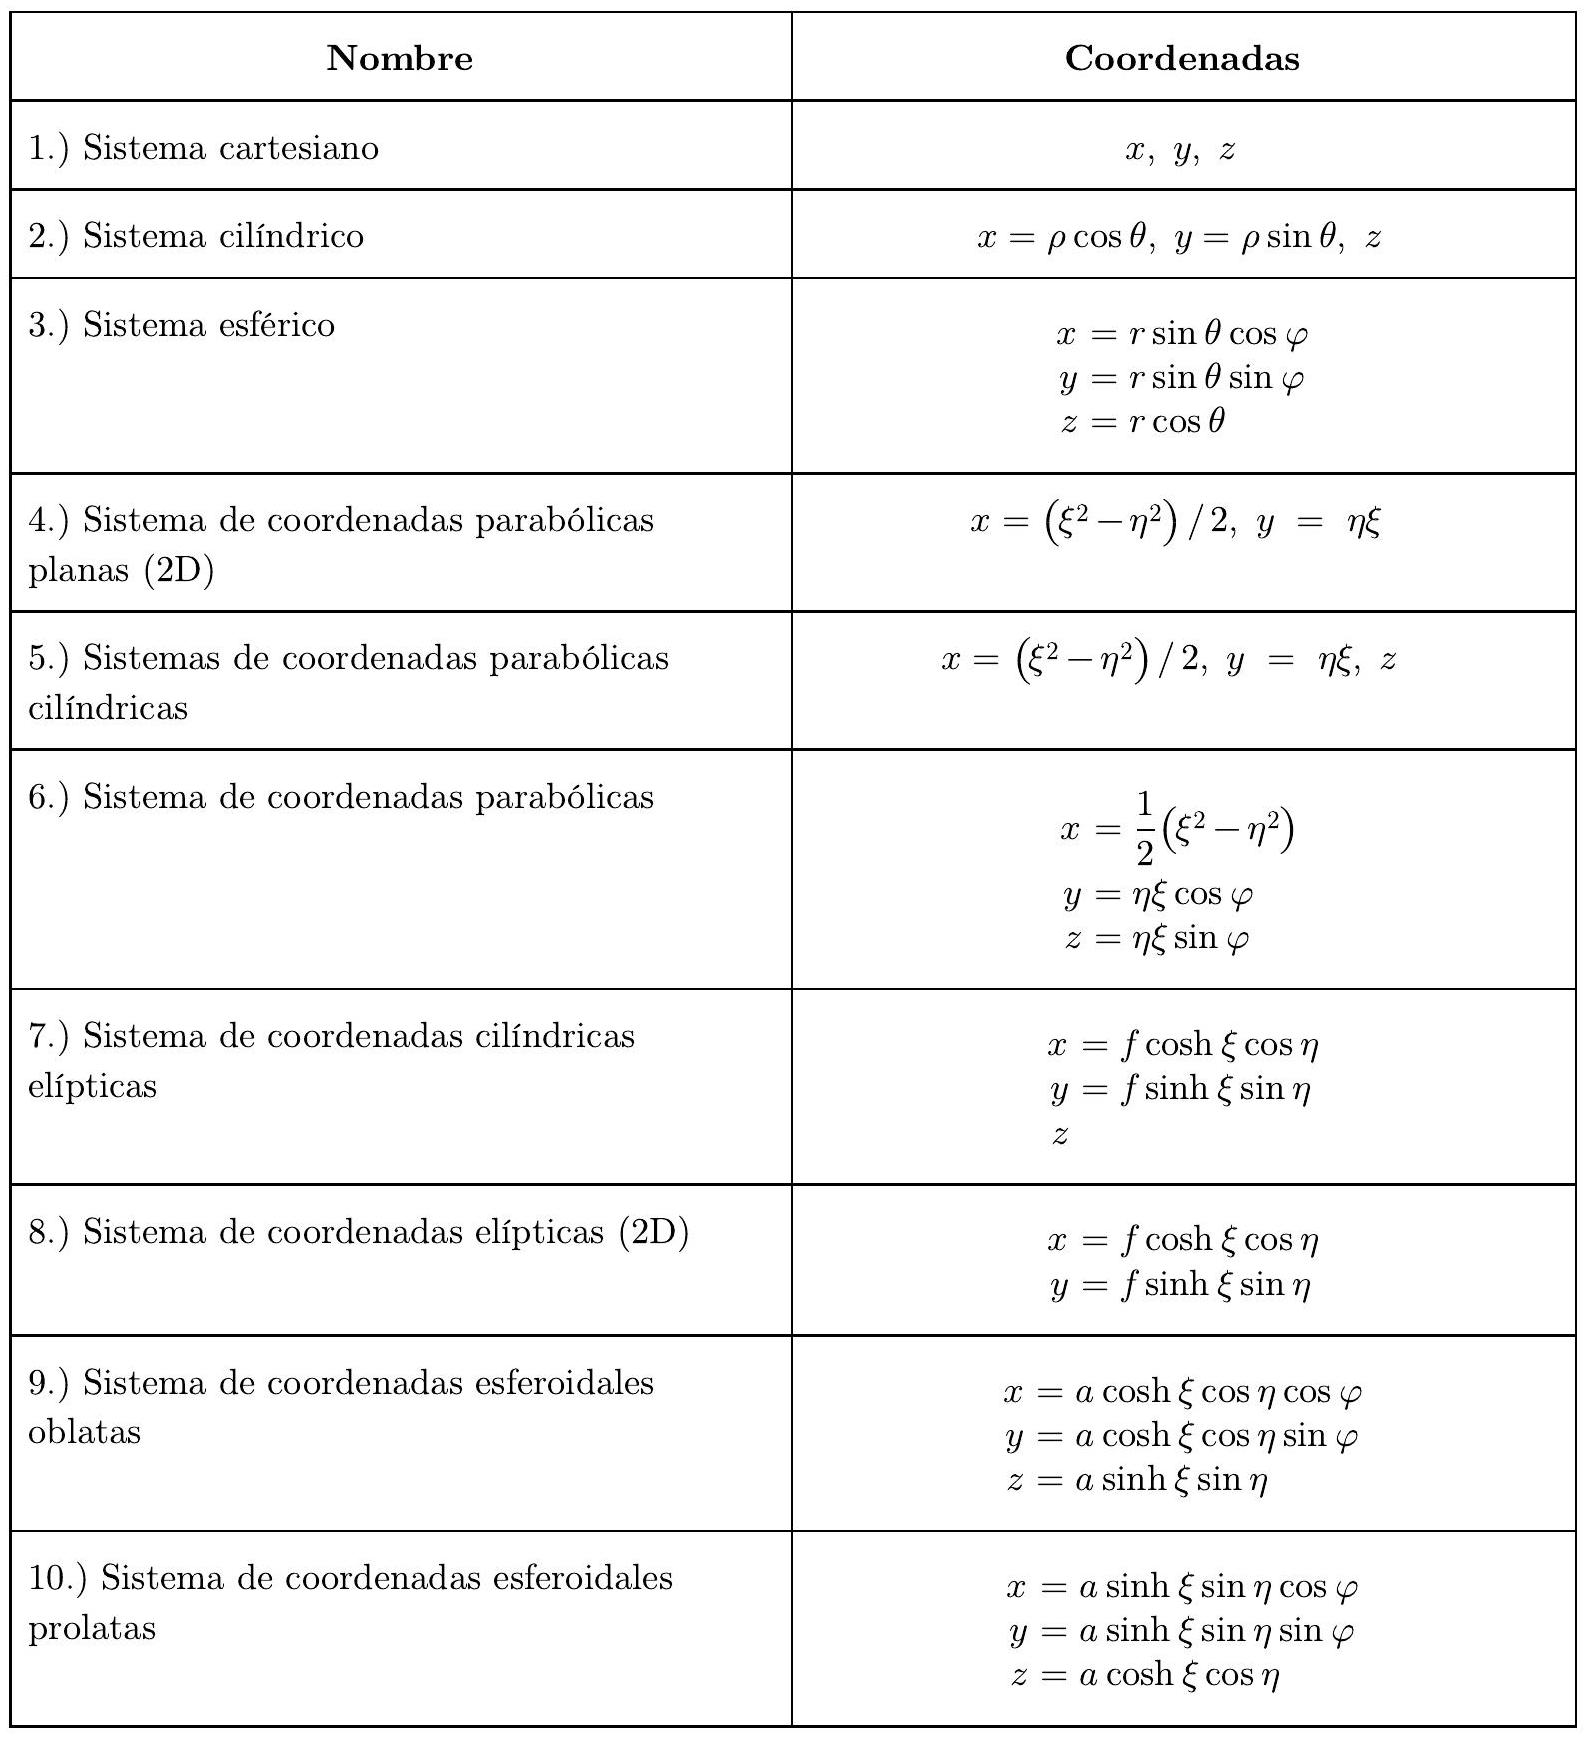
\includegraphics[max width=\textwidth]{/home/gabo/Documents/PLNotes/chapters/Matemáticas/Sistema de coordenadas/images/2023_01_14_5f03f91587087c6429b1g-3.jpg}
\end{center}

\begin{center}
\begin{tabular}{|l|l|}
\hline
11.) Sistema de coordenadas bipolares & $x=\frac{a \sinh \eta}{\cosh \eta-\cos \xi}$ \\
 & $y=\frac{a \sin \xi}{\cosh \eta-\cos \xi}$ \\
 & $z$ \\
\hline
12.) Sistema de coordenadas toroidales & $x=\frac{a \sinh \eta \cos \varphi}{\cosh \eta-\cos \xi}$ \\
 & $y=\frac{a \sinh \eta \sin \varphi}{\cosh \eta-\cos \xi}$ \\
 & $z=\frac{a \sin \xi}{\cosh \eta-\cos \xi}$ \\
\hline
13.) Sistema de coordenadas biesféricas & $y=\frac{a \sin \xi \cos \varphi}{\cosh \eta-\cos \xi}$ \\
 & $y=\frac{a \sin \xi \sin \varphi}{\cosh \eta-\cos \xi}$ \\
 & $z=\frac{a \sinh \eta}{\cosh \eta-\cos \xi}$ \\
\hline
\end{tabular}
\end{center}

Cada sistema coordenado tendrá un dominio para cada una de sus variables, de modo que queden cubiertos todos los puntos del plano o el espacio según sea la situación.

Consideremos ahora la siguiente situación general, si $x=x\left(u_{1}, u_{2}, u_{3}\right), y=y\left(u_{1}, u_{2}, u_{3}\right)$ y $z=z\left(u_{1}, u_{2}, u_{3}\right)$, del cálculo diferencial

$$
\begin{aligned}
& d x=\frac{\partial x\left(u_{1}, u_{2}, u_{3}\right)}{\partial u_{1}} d u_{1}+\frac{\partial x\left(u_{1}, u_{2}, u_{3}\right)}{\partial u_{2}} d u_{2}+\frac{\partial x\left(u_{1}, u_{2}, u_{3}\right)}{\partial u_{3}} d u_{3} \\
& d y=\frac{\partial y\left(u_{1}, u_{2}, u_{3}\right)}{\partial u_{1}} d u_{1}+\frac{\partial y\left(u_{1}, u_{2}, u_{3}\right)}{\partial u_{2}} d u_{2}+\frac{\partial y\left(u_{1}, u_{2}, u_{3}\right)}{\partial u_{3}} d u_{3} \\
& d z=\frac{\partial z\left(u_{1}, u_{2}, u_{3}\right)}{\partial u_{1}} d u_{1}+\frac{\partial z\left(u_{1}, u_{2}, u_{3}\right)}{\partial u_{2}} d u_{2}+\frac{\partial z\left(u_{1}, u_{2}, u_{3}\right)}{\partial u_{3}} d u_{3}
\end{aligned}
$$

De tal manera,

$$
\begin{aligned}
d \vec{r} & =\frac{\partial \vec{r}}{\partial u_{1}} d u_{1}+\frac{\partial \vec{r}}{\partial u_{2}} d u_{2}+\frac{\partial \vec{r}}{\partial u_{3}} d u_{3} \\
& =\sum_{i=1}^{3} \frac{\partial \vec{r}}{\partial u_{i}} d u_{i}
\end{aligned}
$$

Si se propone que: $\frac{\partial \vec{r}}{\partial u_{i}}=h_{i} \hat{e}_{i}$, entendiendo que la derivada de $\vec{r}$ se escribe en la base de vectores $\left\{\widehat{e}_{i}\right\}$ unitarios. De ahí desprendemos,

$$
h_{i}=\left|\frac{\partial \vec{r}}{\partial u_{i}}\right| \quad \hat{e}_{i}=\frac{1}{h_{i}} \frac{\partial \vec{r}}{\partial u_{i}}
$$

La constante de proporcionalidad $h_{i}$ recibe el nombre de factor de escala.

\section{Ejemplos:}
Encuentre los factores de escala y los vectores unitarios en coordenadas cilíndricas y esféricas.

Escribamos a $\vec{r}$ en coordenadas cartesianas

$$
\vec{r}=x \hat{i}+y \hat{j}+z \hat{k}
$$

Con la transformación: $x=\rho \cos \theta, y=\rho \sin \theta, z$

$$
\begin{aligned}
& \vec{r}=\rho \cos \theta \hat{i}+\rho \sin \theta \hat{j}+z \hat{k} \\
h_{\rho} & =\left|\frac{\partial}{\partial \rho}\{\rho \cos \theta \hat{i}+\rho \sin \theta \hat{j}+z \hat{k}\}\right| \\
= & |\cos \theta \hat{i}+\sin \theta \hat{j}| \\
= & \sqrt{\sin ^{2} \theta+\cos ^{2} \theta} \\
h_{\rho} & =1 \\
h_{\theta} & =\left|\frac{\partial}{\partial \theta}\{\rho \cos \theta \hat{i}+\rho \sin \theta \hat{j}+z \hat{k}\}\right| \\
= & \mid-\rho \sin \theta \hat{i}+\rho \cos \theta \hat{j}\rceil \\
& =\sqrt{\rho^{2}\left(\sin 2 \theta+\cos ^{2} \theta\right)} \\
h_{\theta} & =\rho \\
h_{z}= & \left|\frac{\partial}{\partial z}\{\rho \cos \theta \hat{i}+\rho \sin \theta \hat{j}+z \hat{k}\}\right| \\
& =|1 \hat{k}| \\
h_{z} & =1
\end{aligned}
$$

De esta manera los factores de escala en coordenadas cilíndricas, son:

$$
\left(h_{\rho}, h_{\theta}, h_{z}\right)=(1, \rho, 1)
$$

De acá los vectores unitarios, son: $\left(\widehat{e}_{i}=\frac{1}{h_{i}} \frac{\partial \vec{r}}{\partial u_{i}}\right)$

$$
\begin{aligned}
\widehat{e}_{\rho} & =\frac{1}{h_{\rho}} \frac{\partial \vec{r}}{\partial \rho} \\
& =\frac{\partial \vec{r}}{\partial \rho} \quad\left(\text { ya que } h_{\rho}=1\right) \\
& =\frac{\partial}{\partial \rho}\{\rho \cos \theta \hat{i}+\rho \sin \theta \hat{j}+z \hat{k}\} \\
\hat{e}_{\rho} & =\cos \theta \hat{i}+\sin \theta \hat{j}
\end{aligned}
$$

$$
\begin{aligned}
\hat{e}_{\theta} & =\frac{1}{h_{\theta}} \frac{\partial \vec{r}}{\partial \theta} \\
& =\frac{1}{\rho} \frac{\partial}{\partial \theta}\{\rho \cos \theta \hat{i}+\rho \sin \theta \hat{j}+z \hat{k}\} \\
\hat{e}_{\theta} & =-\sin \theta \hat{i}+\cos \theta \hat{j} \\
\widehat{e}_{z} & =\frac{1}{h_{z}} \frac{\partial \vec{r}}{\partial z} \\
& =\frac{\partial \vec{r}}{\partial z}\left(\text { ya que } h_{z}=1\right) \\
& =\frac{\partial}{\partial z}\{\rho \cos \theta \hat{i}+\rho \sin \theta \hat{j}+z \hat{k}\} \\
\hat{e}_{z} & =\hat{k}
\end{aligned}
$$

Por lo tanto

$$
\left\{\widehat{e}_{\rho}, \hat{e}_{\theta}, \hat{e}_{z}\right\}=\{\cos \theta \hat{i}+\sin \theta \hat{j},-\sin \theta \hat{i}+\cos \theta \hat{j}, \hat{k}\}
$$

De donde podemos constatar que:

$$
\begin{aligned}
\widehat{e}_{\rho} \cdot \hat{e}_{\theta} & =(\cos \theta \hat{i}+\sin \theta \hat{j}) \cdot(-\sin \theta \hat{i}+\cos \theta \hat{j}) \\
& =-\sin \theta \cos \theta+\sin \theta \cos \theta \\
& =0 \\
\hat{e}_{\rho} \cdot \widehat{e}_{z} & =(\cos \theta \hat{i}+\sin \theta \hat{j}) \cdot(\hat{k}) \\
& =0 \\
\widehat{e}_{\theta} \cdot \hat{e}_{z} & =(-\sin \theta \hat{i}+\cos \theta \hat{j}) \cdot(\hat{k}) \\
& =0
\end{aligned}
$$

$\mathrm{Y}$

$$
\begin{aligned}
& \hat{e}_{\rho} \cdot \hat{e}_{\rho}=(\cos \theta \hat{i}+\sin \theta \hat{j}) \cdot(\cos \theta \hat{i}+\sin \theta \hat{j}) \\
& =\cos ^{2} \theta+\sin ^{2} \theta \\
& =1 \\
& \widehat{e}_{\theta} \cdot \hat{e}_{\theta}=(-\sin \theta \hat{i}+\cos \theta \hat{j}) \cdot(-\sin \theta \hat{i}+\cos \theta \hat{j}) \\
& =\sin ^{2} \theta+\cos ^{2} \theta \\
& =1 \\
& \hat{e}_{z} \cdot \hat{e}_{z}=(\hat{k}) \cdot(\widehat{k}) \\
& =1
\end{aligned}
$$

Lo cual muestra que se tiene una base de vectores unitarios y ortogonales $\left(\hat{e}_{\rho}, \hat{e}_{\theta}, \hat{e}_{z}\right)$. También se puede verificar que es un sistema de mano derecha. Verifiquemos que $\widehat{e}_{\rho}=\hat{e}_{\theta} \times \hat{e}_{z}$

$$
\begin{aligned}
\hat{e}_{\theta} \times \widehat{e}_{z} & =\left|\begin{array}{ccc}
\hat{i} & \hat{j} & \hat{k} \\
-\sin \theta & \cos \theta & 0 \\
0 & 0 & 1
\end{array}\right| \\
& =(\cos \theta-0) \hat{i}-(-\sin \theta-0) \hat{j}+(0-0) \hat{k} \\
& =\cos \theta \hat{i}+\sin \theta \hat{j}
\end{aligned}
$$

Como $\hat{e}_{\rho}=\cos \theta \hat{i}+\sin \theta \hat{j}$, entonces

$$
\hat{e}_{\rho}=\hat{e}_{\theta} \times \hat{e}_{z}
$$

De manera análoga:

$$
\hat{e}_{\theta}=\widehat{e}_{z} \times \widehat{e}_{\rho}
$$

Calculemos:

$$
\begin{aligned}
\hat{e}_{z} \times \hat{e}_{\rho} & =\left|\begin{array}{ccc}
\hat{i} & \hat{j} & \hat{k} \\
0 & 0 & 1 \\
\cos \theta & \sin \theta & 0
\end{array}\right| \\
& =(0-\sin \theta) \hat{i}-(0-\cos \theta) \hat{j}+(0-0) \hat{k} \\
& =-\sin \theta \hat{i}+\cos \theta \hat{j}
\end{aligned}
$$

Como $\hat{e}_{\theta}=-\sin \theta \hat{i}+\cos \theta \hat{j}$, entonces se ha verificado que: $\hat{e}_{\theta}=\hat{e}_{z} \times \hat{e}_{\rho}$.

Finalmente verifiquemos que: $\widehat{e}_{z}=\widehat{e}_{\rho} \times \widehat{e}_{\theta}$

$$
\begin{aligned}
\widehat{e}_{\rho} \times \widehat{e}_{\theta} & =\left|\begin{array}{ccc}
\hat{i} & \hat{j} & \hat{k} \\
\cos \theta & \sin \theta & 0 \\
-\sin \theta & \cos \theta & 0
\end{array}\right| \\
& =(0-0) \hat{i}-(0-0) \hat{j}+\left(\cos ^{2} \theta+\sin ^{2} \theta\right) \hat{k} \\
& =\widehat{k}
\end{aligned}
$$

Por lo tanto $\hat{e}_{z}=\hat{e}_{\rho} \times \hat{e}_{\theta}$

\section{Tarea:}
\begin{itemize}
  \item Realizar todo lo anterior para las coordenadas esféricas, es decir, encontrar factores de escala, vectores unitarios, probar su ortogonalidad, unitariedad y regla de la mano derecha.

  \item Tomar las coordenadas esferoidales oblatas y hacer todo lo anterior.

\end{itemize}
